\documentclass[12pt, a4paper]{report}

\usepackage{fyp}


%%these packages are not really necessary if you dont need the code and proofs environments
%%so if you like you can delete from here till the next comment
%%note that there are some examples below which obviously won't work once you remove this part
\usepackage{verbatim}
\usepackage{amsfonts}
\usepackage{amsmath}
\usepackage{amssymb}
\usepackage{amsthm}

\usepackage{pdfpages}
\usepackage{amssymb}
\usepackage{graphicx}
\usepackage{listings}
\usepackage{proof}
\usepackage{xcolor}
\usepackage{titlesec}
\usepackage{rotating}
\usepackage{float}
\usepackage{tikz}
\usepackage{url}

\definecolor{OliveGreen}{rgb}{0,0.6,0}


\lstset{
  language=C,
  frame=tb,
  aboveskip=3mm,
  basicstyle=\footnotesize\ttfamily,
  numbers=left,
  stepnumber=1,
  numbersep=10pt,
  tabsize=4,
  columns=flexible,
  numbers=none,
  numberstyle=\tiny\color{gray},
  keywordstyle=\color{blue},
  commentstyle = \color{OliveGreen},
  stringstyle=\color{purple},
  breaklines=true,
  breakatwhitespace=true,
  showstringspaces=false,
  tabsize=3,
  numbers=left
}

%%the following environments are useful to present proofs in your thesis
\theoremstyle{definition}
\newtheorem{definition}{Definition}[section]
\theoremstyle{definition}%plain}
\newtheorem{example}{Example}[section]
\theoremstyle{definition}%remark}
\newtheorem{proposition}{Proposition}[section]
\theoremstyle{definition}%remark}
\newtheorem{lemma}{Lemma}[section]
\theoremstyle{definition}%remark}
\newtheorem{corollary}{Corollary}[section]
\theoremstyle{definition}%remark}
\newtheorem{theorem}{Theorem}[section]
%%you can delete till here if you dont need the code and proofs environments

\setlength{\headheight}{15pt}
%\overfullrule=15pt

\begin{document}

%%make sure to enter this information
\title{JavaScript Framework for Actor-Based Programming}
\author{Andrew Buhagiar}
\date{\today}
\supervisor{Prof. Kevin Vella}
\department{Faculty of ICT}
\universitycrestpath{crest}
\submitdate{May 20, 2022} 

\frontmatter

\begin{acknowledgements}
I thank Prof.\ Kevin Vella for his continuous support, patience, and advice which allowed me to complete the objectives of this project.

I also extend my gratitude to my family for their investment which allowed me to pursue my studies.

\end{acknowledgements}
       
\begin{abstract}
This dissertation explores the suitability of the actor model when used to bring concurrency and parallelism to JavaScript. Actors are concurrent isolated units of computation which process messages using their predefined behaviour. The implementation takes the form of two APIs for both the Node.js and browser environments respectively, allowing developers to intuitively reason about engineering JavaScript programs through the spawning and sending of messages to actors.

Isolated actors can be safely spawned on remote devices over a network as well as utilise multiple cores on a local processor. This allows for distributed and parallel computation which have the potential of shortening the time taken when executing computationally intensive tasks. A WebSocket~\cite{websocket} server is used to connect a finite number of Node.js instances and browsers hosting actors over the network. Faster communication links are explored using inter-process communication when hosting multiple processes on a local device. The framework abstracts the adaptive use of different communication links and provides location transparency for remote actors.

Benchmarks analyse the framework's performance when used on a single instance using Node.js or a browser, as well as the speedup introduced when utilising additional local or distributed cores working on the same task. The performance of our JavaScript framework is evaluated against existing JVM and JavaScript actor framework implementations. The relative performance of the communication links used when distributing actors is also explored.

Nowadays, browsers are found on devices such as smart fridges and TVs, each of which able to run JavaScript defined behaviour. The increasingly popular Node.js environment for server-side applications would be able to host actors which can communicate with actors hosted on browsers, enabling uniform and flexible scaling of applications. The limitations of the framework are discussed as well as its untapped potential when it comes to freezing and migrating actors across the web.
\end{abstract}

\tableofcontents

\listoffigures

\mainmatter

\chapter{Introduction}
\section{Motivation}
%Why JavaScript
JavaScript~\cite{ecmascript} is widely used for client applications on the browser and benefits from a growing popularity of server-side applications using environments such as Node.js~\cite{nodejs}. It is a single-threaded language which lacks an intuitive way to program in a parallel and distributed fashion. This dissertation presents a prototype that implements a JavaScript framework which allows developers to build actor-based systems. Developers can use actors as concurrent units of computation which can be deployed either locally or remotely on multiple node runtimes and browsers. This will allow developers to intuitively distribute work amongst multiple processors and devices to fully utilise the hardware available in servers and modern computers.

%Why Actors
Actors~\cite{hewitt1973session}\cite{43years} communicate with each other through messages which are stored in the receiving actor's message queue. A message is processed by executing its defined actor behaviour. The Actor Model is a good fit for JavaScript's event loop~\cite{eventloopbrowser}\cite{eventloopnode} as they are both event driven, and has already achieved success in the telecommunications industry and is more recently used for implementing distributed systems in languages such as Erlang and Scala/Akka~\cite{haller2012integration}.

%The Frameworks
JavaScript allows developers to import exported variables and functions from different files. The developed prototype takes the form of multiple frameworks for the browser and Node.js environments respectively. The frameworks' APIs will abstract the prototype's internal mechanisms which spawn and interact with actors, allowing developers to intuitively make use of the actor model in their code. Frameworks will be provided for the browser and Node.js environment respectively

\section{Objectives}
This dissertation will explore the suitability of the Actor Model when used to reason about distributed and concurrent systems in JavaScript through the use of the developed frameworks. The frameworks' suitability is based on its performance, scalability, and intuitiveness to use. The objectives of the artifact are as follows.
\begin{enumerate}
    \item Allow developers to easily define and spawn actors through the framework API on Node.js or a browser. Actors should be able to send messages to each other as well as spawn more actors. Full interoperability should be provided when using the framework across the two environments.
    \item Allow for spawning and interacting with actors on different Node.js instnaces and browsers through different network links. Node.js cluster\cite{cluster} can be used for IPC between node processes, while Web Workers\cite{webworkers} can be used for communication between the primary thread and its spawned workers. When such communication links are not available, the network stack is involved by using WebSockets for flexible communication to link remote processes and devices.
    \item Provide location transparency when dealing with actor references. Interacting with a local actor should be the same as interacting with a remote actor when using the API.
    \item Benchmark the performance and scalability of the developed prototype as well as evaluate its practicality.
\end{enumerate}

Chapter 2 contains the background and literature review. The design and implementation details are covered in Chapter 3, followed by benchmarks and evaluation in Chapter 4. Chapter 5 contains the conclusions and future work.

\chapter{Background and Literature Review}
\section{Concurrency and Parallelism on JavaScript}
Concurrency allows one to switch the order of the execution of tasks without yielding a different output. Since the order in which a program is executed would not an issue, one can run these code segments in parallel, potentially reducing the time taken to process a particular task. JavaScript relies on a single-threaded non-blocking event loop~\cite{eventloopbrowser}\cite{eventloopnode} which does not support parallel execution of such tasks, raising an issue when high performance computing~\cite{highperformance} is required. If JavaScript had to block when input or output was required, it would stop a page from being responsive. Instead, JavaScript handles I/O using events and callback functions which are posted on the event queue. The event loop processes each of the events in FIFO order, where each event has a corresponding callback or event listener function to execute. Each message is processed to completion without pre-emption by the processing of a different message, allowing for consistent concurrency when executing the same code segment. Browser Web Workers\cite{webworkers} and Node.js child processes\cite{cluster} can be used to bring parallel computation to JavaScript~\cite{concurrencyjs}\cite{spidersjs}. They adopt a similar philosophy to that of the actor model as both involve isolated instances which communicate through messaging to collaborate when working on computationally intensive tasks.

JavaScript allows developers to make use of Promises~\cite{promises} as a replacement for executing callback functions after finishing a task. A Promise object takes in a function as parameter which includes the task that is to be executed. This function will have a `resolve' and `reject' parameter which can be called upon the successful or failed completion of the task. Developers can create functions which return a Promise and then define how to `consume' the returned promise. Different behaviour can be defined if the promise succeeds, such as consuming the returned data through the use of another callback function. One can also handle the event of a promise's failure, much like catching an exception. JavaScript later developed the async/await syntax~\cite{async} where async functions always return a promise resolving into the value that is returned by the function. An await expression suspends the execution of an async function until the promise can be consumed, eliminating the need to define promise chains.

JavaScript is an implementation of the ECMAScript design. The ECMA-262 language has multiple published editions, each of which serving as the blueprint for Javascript's next stable release. ECMAScript 8~\cite{ecmascript} provides the SharedArrayBuffer~\cite{sharedarraybuffer} constructor which allows for concurrent access for a set of bytes. This allows for memory to be shared across agents in different cluster processes or web workers. The process which created the SharedArrayBuffer need only pass the object to the workers to allow them to access and manipulate the same data block. SharedArrayBuffers allow for different workers to have access to the same memory which promotes collaboration when working on the same data points. However, multiple workers manipulating the same data may lead to data races and additional care must be taken by the developer.

\section{The History of the Actor Model}
The Actor Model was first introduced by Carl Hewitt~\cite{hewitt1973session}\cite{43years} in 1973 for research in artificial intelligence. It defines actors as computational agents which execute a uniform behaviour when sent a message. Hewitt argued that the actor metaphor can be applied to processes and daemons amongst other things. Two years later, Carl Hewitt helped in writing a draft of PLASMA~\cite{plasma}\cite{chewitthowto}, the first actor model language. In this language, actors communicate with each other using messages and the receiver processes the received message using its pre-defined computation. Based on the message's contents, the actor may choose one from different behaviours which may involve sending messages to other actors.

The actor model was clarified by Gul Agha~\cite{agha1985actors} in 1986. While Carl Hewitt's paper set the foundation of the potential applications of the actor metaphor, Gul Agha focused on how actors can be used to create expressive, simple, and intuitive programming languages. Gul Agha believed that it is more cost effective to use many smaller processors rather than rely on an individual powerful processor. His paper focused on the linguistic issues of a programming language which made concurrency intuitive when reasoning about collaborating processors. Gul Agha identified actors as computational agents which map incoming messages to a behaviour. Such behaviour may include communicating with other actors, deciding how the next incoming communication will be processed as well as creating more actors. Gul Agha favoured buffered asynchronous communication when it came to sending messages as it allows an actor to communicate with itself without waiting, as well as to promote efficient use of the processing power rather than wait for the receiver to accept communication. Gul Agha also recognised the fact that delivery of messages is not guaranteed on a network, and that all receiving buffers are bounded.

In the same year as Gul Agha's paper was made public, a programming language called Erlang~\cite{erlang} made its first appearance. It was designed to address the highly concurrent nature of telephony applications. A high degree of fault tolerance was at the core of Erlang's design to minimise failure in telephone systems when changing the system's software. Erlang uses the actor model to allow for concurrent programming, such that each independent process communicates with other processes through the sending of messages. This makes `actors' and Erlang's lightweight `processes' interchangeable in the remaining discussion of Erlang. Each process has a FIFO mailbox (queue) which processes the messages in the order they were received. Erlang adopts asynchronous message passing, promoting developers to send messages without blocking. The language is also designed to let processes crash, as external processes can easily observe each other. When a process which provides the service crashes, the monitoring process can take over and resume the service. Erlang was continuously updated and found success in large scale mobile networks thanks to the actor model's potential to build reactive systems\cite{reactivemanifesto}. Erlang processes allow for elastic systems such that one can add more processes to address a larger workload, while monitoring processes allows for fault tolerance and responsiveness of the system. 

Nowadays, several variants of the actor model are used to fit the requirements of modern languages and frameworks. Popular languages such as Scala~\cite{scala} with Akka~\cite{akka} and Elixir~\cite{elixir} (built on top of Erlang) use the actor model to allow developers to build scalable and distributed systems.

\section{Similar Work}
Several JavaScript frameworks which implement the actor model are available on the node package manager (npm) and in public git repositories.

\textbf{Clooney}~\cite{clooney} is described as an actor library for the browser by the Google Chrome team. It offers an API which takes in classes with methods which will be instantiated in Web Workers~\cite{webworkers}. Developers can call the defined functions inside the actors as if they were a regular class. This library abstracts away the use of Web Workers when parallelising work.

\textbf{Nact}~\cite{nact} is a faithful implementation to the actor model as it also relies on message passing for communication between spawned isolated actors. One spawns an actor by first defining the actor's behaviour through a function with the state, message and system context as the parameters. The function will be called for every message that is sent to the spawned actor. The framework does not seem to have in built functionality to communicate with actors over the web, as it makes use of a JavaScript REST API to expose actors to the web in one of the provided examples.

\textbf{Akka.js}~\cite{stivan2015akka} allows developers to port Akka programs to JavaScript browsers and server-side runtimes. This framework allows developers to build distributed applications on separate browsers using WebRTC~\cite{webrtc} for communication. It also allows developers to only make use of Scala~\cite{scala} to deploy actors on both browsers and servers.

\textbf{Spiders.js}~\cite{spidersjs} identifies the problem of different API's being used for web workers and child processes, both of which are inspired by the actor model for constructing parallel systems using JavaScript. This project is focused on defining a single actor model API no matter if it's a client or server-side application. The paper benchmarks the usage of Spiders.js against JavaScript native web workers as well as the actor creation overhead for both. This framework allows for communication with actors over a network when provided the machine's IP address and port number it is listening on. Spiders.js spawns a new Node.js child process/web worker for each actor to provide each actor with its own thread of control, allowing developers to engineer systems using Communicating Event Loops (CEL).

\textbf{TigerQuoll}~\cite{tigerquoll} took a different approach when providing parallelism to the language. It acknowledged the actor model as too limited for the requirements of more complex patterns that occur in modern applications. Instead it allows developers to use regular event based programming to register events for parallel processing. Kurt Micallef's paper~\cite{kurt} also brings parallelism to JavaScript by exploiting ES6 Generators and several web technologies. His prototype allows for developers to engineer parallel and distributed programs over both browsers and Node.js, provided that development is done through the use of Communicating Sequential Processes (CSP).

\chapter{Design and Implementation}
\section{Framework Design}
\subsection{Introduction}
\begin{figure}[H]
    \begin{centering}
        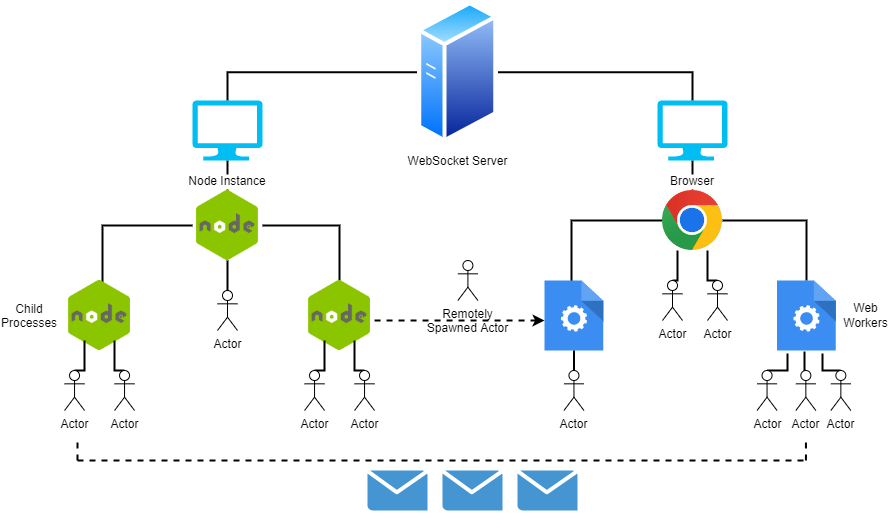
\includegraphics[width=\textwidth]{resources/network.png}
        \caption{A Network of Devices with Multiple Processes Hosting Actors}
    \end{centering}
\end{figure}
This section delves into the framework's design through a series of subsections which cover parts of the system. Two APIs are developed for Node.js and browsers separately while providing full interoperability. The API provides functions to JavaScript developers which allow for the engineering of actor-based systems. The framework's design reflects the objectives defined in Chapter 1. Referring to the figure above, the framework's design will enable actors to coexist in both Node.js and browser instances across local or remote devices. The API must be intuitive while also enabling the engineering of flexible actor-based systems.
\subsection{Actors}
The design of the frameworks' actors is inspired by Gul Agha's~\cite{agha1985actors} definition in 1985. They are defined as computational agents which map communication to a behaviour which may consist of spawning new actors, communicating with other actors or defining a new behaviour for the next message. The behaviour of such actors is also said to be history sensitive, where previous behaviour executions may impact how the next communication is processed.

Agha's definition prompts the API to allow for the creation of actors and the ability to send communications to the spawned actors. Communications sent to actors will take the form of JavaScript objects due to their structural flexibility and conformity with Agha's definition of a “tuple of values”. The actor's history sensitivity prompts for each actor to hold a local and isolated state which will also take the form of a JavaScript object. The actor's behaviour will take the form of a conventional JavaScript callback function, which will have the actor's state, message and self address as function parameters. Since JavaScript provides first class functions, the behaviour definition can be stored and called when required. This prompts for the following basic API using TypeScript's~\cite{typescript} notation.
\begin{lstlisting}
interface ActorBehaviour {
    (state: object, message: object, self: ActorReference): void
}
spawn = (initialState: object, behaviour: ActorBehaviour): ActorReference
send = (actor: ActorReference, message: object): void    
\end{lstlisting}
The API will return an actor reference when one is spawned, which can then be fed into the send function as a parameter. The actor behaviour will be invoked when processing each received message and may manipulate the actor's state which is first defined as a parameter when invoking spawn function. The actor behaviour may also use the API to spawn and communicate with other actors. The implementation of these two functions on the Node.js and browser environment will fulfil the first defined objective in the introduction section. 
\begin{figure}[H]
    \begin{centering}
        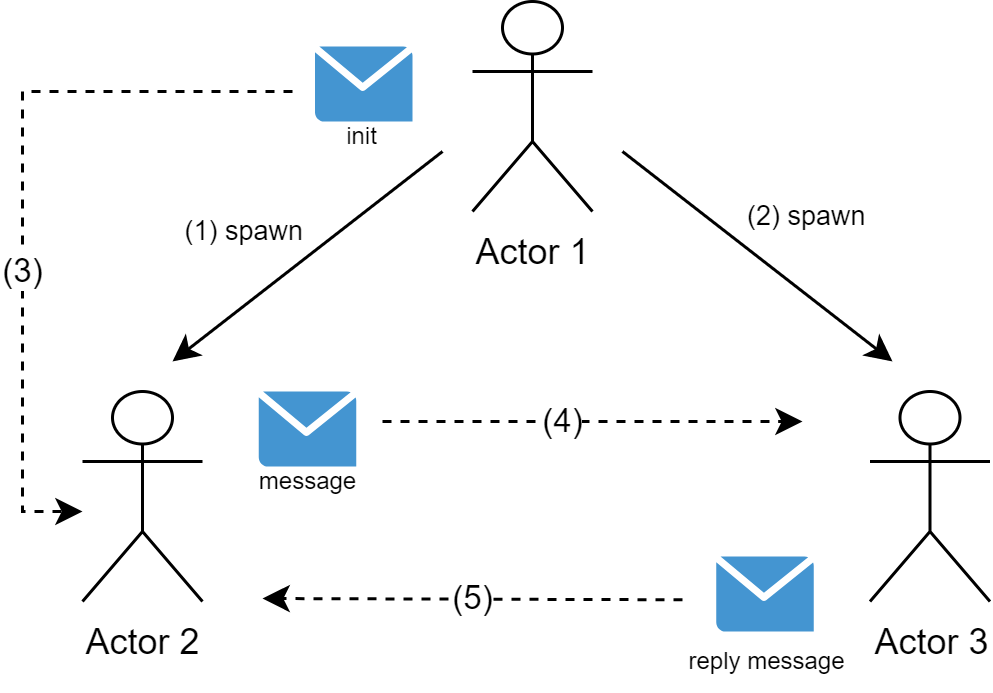
\includegraphics[width=270px]{resources/actors.png}
        \caption{Spawning Actors and Sending Messages}
    \end{centering}
\end{figure}
Finally, a function to terminate an actor is provided, with the option for whether it should process the remaining messages. This function takes in an actor reference similar to the send function.
\begin{lstlisting}
terminate = (actor: ActorReference, force: boolean)
\end{lstlisting}
\subsection{Intuitive Networking}
So far, the design of the actors allows for concurrent processing of messages on one browser or Node.js instance. Concurrent programming entails that it does not matter which actor processes their next message, or in which order the actor processes their messages, assuming that the actors are not overly dependent on their maintained isolated state. Concurrency implies that actors are potentially parallelisable, where multiple actors can process their next message in parallel and thus having the potential to speed up the overall computation. The API must provide an intuitive way to establish a connection with other processes or devices as well to communicate with remote actors.

A peer-to-peer system was first considered to connect nodes which host actors. Each peer would have a list of nodes to establish connection with. While this would eliminate the additional network hop introduced by an intermediate server, the number of connections performed would be $n!$ if each node is listening for connections and connects to every other node. Furthermore, manually entering which peers each node needs to establish connection with is tedious. The prototype instead opts for a central WebSocket server for distributed networking, as each node can communicate with the rest of the network which only requires $n$ connections.

The WebSocket server expects a finite number of $n$ connected clients before it starts accepting communication to be forwarded between nodes. The server logic was developed separate from the actor framework and assumes that connections are not terminated in the duration of its runtime. The WebSocket server will assign a unique identifier to each connected client which will be broadcasted when the server has the expected number of connected clients. This will allow developers to specify a particular node when utilising the framework.

\begin{figure}[H]
    \begin{centering}
        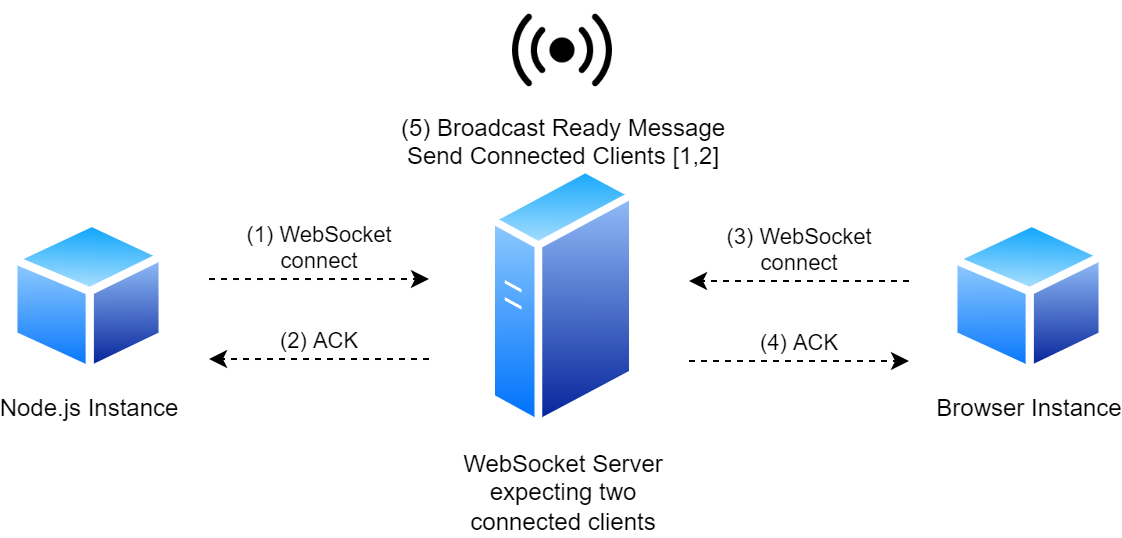
\includegraphics[width=350px]{resources/websocketconnection.png}
        \caption{WebSocket Server Connecting Node.js Instance to a Browser}
    \end{centering}
\end{figure}
 
This mode of establishing communication between nodes has several advantages and disadvantages. The centralised WebSocket server is effectively creating a barrier which will be lifted when the expected number of clients are connected and can communicate with each other. Once the number of expected clients connect, each client is granted communication with the entire network at the cost of one additional network hop over peer-to-peer. The centralised server also simplifies the logic of uniquely identifying each connected client, which will be a simple iterative naming scheme in the order in which clients connect. Connecting to the server should take the form of an API function call which returns a promise resolving when the server broadcasts to the client that it is ready to forward information to the other connected clients.
\begin{lstlisting}
init = (url: string, timeout:number): Promise<object>
\end{lstlisting}
When the promise is resolved, the developer must be able to refer to actors which exist in remote nodes. API functionality to remotely spawn actors on other nodes would address this requirement as it would allow for one instance to get references to actors it remotely spawned. Security is an issue since actors can be spawned on machines remotely by malicious peers. However, it allows for expressive programs which can centrally load balance work on a distributed network by sending messages to the remote actors using the obtained references through remote spawning.
\begin{lstlisting}
spawnRemote = (node: number, state: object, behaviour: ActorBehaviour, timeout: number): Promise<ActorReference>
\end{lstlisting}
\subsection{Local Parallelism}
The WebSocket server provides distribution for any Node.js or browser client wishing to communicate with actors hosted on other connected clients. However, a developer might want to host multiple instances on a local device to make up for JavaScript's single-threaded nature when distributing actors. The WebSocket server involves an intermediary network hop as well as the network layer, both of which can be avoided by using Node.js~\cite{nodejs} cluster and browser Web Workers~\cite{webworkers}. These methods rely on inter-process communication (IPC) with no network layer and taking advantage of shared memory, while also allowing direct communication between the spawner and the workers. Each of the spawned workers can also be treated as separate instances when connected to the WebSocket server for communication with remote devices.

\begin{figure}[H]
    \begin{centering}
        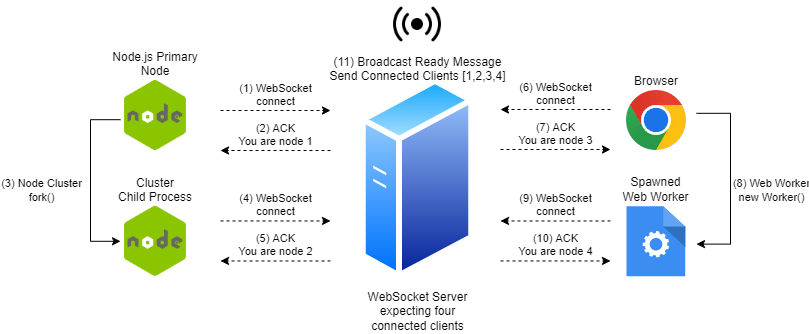
\includegraphics[width=\textwidth]{resources/websocketconnectioncomplex.png}
        \caption{WebSocket Server Connecting Different Types of Processes}
    \end{centering}
\end{figure}

This would require changing the API's init function to allow the developer to specify the number of additional workers to spawn and connect to the WebSocket server, resulting in the function definition below.
\begin{lstlisting}
init = (url: string, timeout: number, numWorkers: number = 0): Promise<object>
\end{lstlisting}
The default number of workers set to 0, where the instance would not spawn any workers. Implementation of the networking logic which would allow actors to communicate over a network would satisfy the second defined objective for this dissertation.
\subsection{Location Transparency}
Now that Node.js Cluster child processes and browser Web Workers have been introduced and incorporated into the API's design, the send function would benefit from location transparency. This would mean that the developer does not need to specify whether the actor resides in a spawned Web Worker or Node.js child process, as well as whether it is a local or remote actor. This is done by first embedding in which node the actor resides in as well as the actor's unique name inside the actor reference returned by the API's spawning functions.
\begin{lstlisting}
interface ActorReference {
    name: string,
    node: number
}
\end{lstlisting}
Using this, the send function should determine which communication link to use based on whether the actor is local, a spawned child process or over the web.
\begin{figure}[H]
    \begin{centering}
        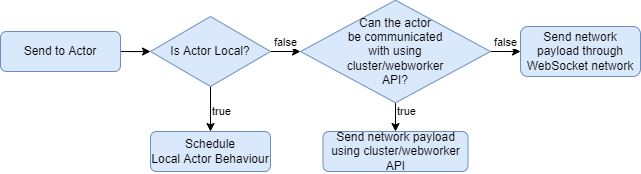
\includegraphics[width=\textwidth]{resources/communication.png}
        \caption{Flowchart for Choosing which Link based on Actor Location}
    \end{centering}
\end{figure}
Using the above decision tree, the framework can internally use the fastest available link when given the node in which the actor resides in.
\subsection{Finalised API}
The next section will cover implementation details of note regarding the API which consists of the following functions.
\begin{lstlisting}
init = (url: string, timeout: number, numWorkers: number): Promise<object>
closeConnection = ()    //Function to close network connection
spawn = (state: object, behaviour: ActorBehaviour | string): ActorReference
spawnRemote = (node: number, state: object, behaviour: ActorBehaviour, timeout: number): Promise<ActorReference>
send = (actor: ActorReference, message: object): void
terminate = (actor: ActorReference, force: boolean = false)
\end{lstlisting}
\section{Implementation}
\subsection{Anatomy of an Actor}
The internal composition of an actor inside the framework is at the heart of the API's features. An actor takes the form of an object which contains its maintained state as well as its behaviour as an executable function. Each actor stores a name so that it can be uniquely identified in the local instance. The network number assigned by the WebSocket server as well as whether the actor is accepting messages is also stored. The TypeScript interface below defines what an actor is composed of.
\begin{lstlisting}
//TypeScript object interface for an Actor
interface Actor {
    name: string,                       //generated using uuidv4
    node: number,                       //found in global variable
    state: { [key: string]: any },      //given by developer
    behaviour: ActorCallback,           //given by developer
    active: boolean                     //starts with true
}
\end{lstlisting}
When spawning an actor, the state and behaviour are defined by the developer. The name is automatically generated using a uuidv4 package~\cite{uuidv4}. All actors start off as active to indicate that they accept messages. When returning the actor reference to the developer, an issue arises if the whole actor object is returned. Not only does it contain redundant information such as returning the state and behaviour that were just defined by the developer, it also undermines the concept of actor isolation. Since objects are passed by reference in JavaScript, the developer or other actors would be able to modify the actor's state and behaviour through its reference. To protect these attributes, only a subset of them are returned, defined by the ActorReference TypeScript interface.
\newpage
\begin{lstlisting}
interface ActorReference {
    name: string,   //identifies the actor on a local instance
    node: number    //identifies the client over the network
}
\end{lstlisting}
\subsection{Communicating with an Actor}
Using the returned ActorReference object from the \textbf{spawn} function, an actor can be uniquely identified across the web. The developer can put in the actor reference inside the \textbf{send} function to send that actor a message. Internally, the framework looks at the actor reference's node number. If it matches the client's network number it resides in, then it will queue the local actor's behaviour on the runtime's event queue. If the actor resides in a remote node, it creates a payload to send over the network. 

When the \textbf{init} function is called, the developer can choose to spawn a number of child processes or web workers. Each of the spawned workers will send to the spawner (primary node) the network number assigned to them by the WebSocket network. The primary node will then send each of the spawned workers of their neighbouring spawned processes' network numbers. This is so that spawned processes can communicate with each other by sending messages to the primary node, which will forward the message to the destination worker using the cluster or web worker API instead of the WebSocket network to avoid the network stack. If the actor resides on a separate device or group of spawned processes, it resorts to using the WebSocket network.
\subsection{Remote Spawning Mechanism}
The \textbf{spawnRemote} function sends a request to spawn an actor to the remote node. The request has embedded within it the string representation of its behaviour which is reconstructed as a function on the recipient end. Similar to the \textbf{send} function, it chooses the fastest transport mechanism to send the spawn request. The primary node is internally aware of the network numbers of the worker nodes it spawned, so it will make use of Cluster IPC to send these requests rather than the slower established WebSocket link through the network.

On the recipient side, the node will spawn an actor with the sent behaviour and initial state. It locally generates the spawned actor's name and embeds it in an acknowledgement sent to the remote spawner. Once this acknowledgement is received by the spawner, it constructs the actor reference using the received actor name and resolves the promise.
\subsection{Actor Runtime}
The JavaScript event loop is responsible for executing the application code. The language's runtime has a queue of messages where each message is mapped to a function which processes that message. The event loop waits for the arrival of a message and processes the queue of messages when there is a backlog in the event queue. Each message is processed to completion before other messages are processed. The Actor Model also maps messages onto functions which act as message handlers. Therefore, the framework's implementation takes advantage of the similar philosophies between the JavaScript runtime and the Actor Model.

The implementation acts as a wrapper of the JavaScript event loop. Once a message is received by an actor, it will schedule the processing of the message on the JavaScript event loop. This is done by scheduling a microtask~\cite{microtasks} which is an event queued to execute before the start of the next event loop~\cite{eventloopbrowser}\cite{eventloopnode}. The microtask is scheduled by creating a promise which is immediately resolved. This behaviour is similar to using Node.js' \textbf{process.nextTick()}~\cite{nexttick} which is more efficient than using the JavaScript's \textbf{setTimeout()} function as it would otherwise schedule a macrotask which executes in the following iteration of the event loop.
\begin{lstlisting}
//Code which schedules the processing of a received message
Promise.resolve().then(() => {
    if (message !== undefined && localActor.active)
        localActor.behaviour(localActor.state, message, { name: localActor.name, node: localActor.node });
})
\end{lstlisting}

Since JavaScript only has one microtask event queue, the order in which messages are sent matches the order in which they are processed by the set of receiving actors. Since JavaScript processes microtasks to completion before processing the next, the implementation ensures that at most one actor is processing a message at any point in time in a single Node.js or browser instance.
\chapter{Evaluation}
This chapter evaluates the developed prototype's performance when executing computationally intensive tasks. Savina~\cite{savina} is a benchmark suite defined for actor-based systems which is partially implemented for this chapter. Section 1 will explore each of Savina's micro-benchmarks which measure overheads introduced when using the framework's basic functionality. Section 2 explores parallel benchmarks which expect a linear increase in performance with each added core. 

Unless otherwise stated, the following hardware and software was used to run the benchmarks.
\begin{itemize}
    \item OS --- Ubuntu 20.04 focal (64 bit)
    \item CPU --- Intel Core i7--1065G7. 4 cores up to 3.9GHz with hyper-threading disabled
    \item RAM --- LPDDR4 16GB (2$\times$8GB) at 4267MHz
    \item Node.js – v16.14.0
    \item Google Chrome v100.0.4896.88 (Official Build)
\end{itemize}

\section{Micro-Benchmark Performance}
\subsection{Comparing Local Node.js to Browser Performance}
The Savina benchmark suite define micro-benchmarks which test specific actor runtime features. The diagram below compares the execution times between the browser and Node.js implementations of Savina's micro-benchmarks. The diagram is followed by an explanation and analysis of each of the executed benchmarks from left to right.
\begin{figure}[H]
    \begin{centering}
        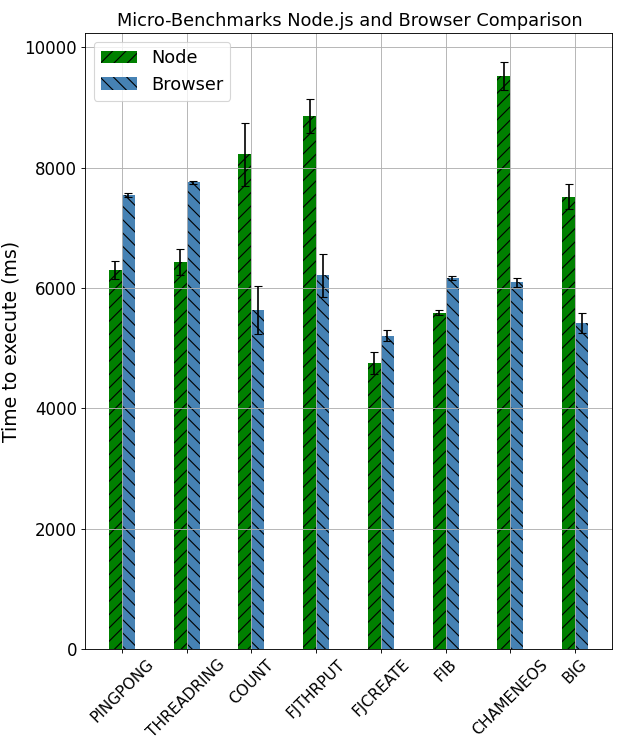
\includegraphics[width=270px]{resources/micro.png}
        \caption{Node.js and Browser Comparison for Micro-Benchmarks}
    \end{centering}
\end{figure}
\begin{itemize}
    \item Ping Pong – Two actors are spawned which will send messages to each other. Every time one actor receives the message, it decrements the integer value it receives and sends it back to the sender. This mainly tests the send functionality on a local instance with Node.js being slightly faster at sending the same load of messages.
    \item Thread Ring – Similar to Ping Pong, the token containing the decrementing integer is now forwarded across N actors. Instead of the message being sent back and forth, it is now forwarded to the next actor on the ring. The performance is nearly identical to that of Ping Pong as the framework does not perform context switching between actors. The JavaScript event loop merely executes the queued functions which process actors' messages. N was set to 10 actors and the initial decrementing integer value (which determines the load) was set to the same as the ping pong benchmark.
    \item Count – This benchmark sends N messages to a single actor and waits for the actor to process all of the sent messages. It tests the time taken for N messages to be sent and then processed by an actor. Since the framework relies on the event loop, each and every sent message gets queued on the event queue. Node is considerably slower than the browser implementation with a high standard deviation on both sides. This may be due to the operating system having to allocate a considerable amount of memory in a short amount of time when queuing a large number of messages.
    \item Fork Join (Throughput) – Similar to the count benchmark, it starts by sending N messages. However, they are sent to K actors in a round robin fashion instead of one counter actor. Similar performance is achieved to that of the count benchmark when sending the same number of messages.
    \item Fork Join (create) – This benchmark creates N actors and sends each spawned actor a single message. It tests the spawning, sending and terminate functionality of the framework by spawning actors and sending one message to each which will cause the actors' termination. The performance is similar between the two environments with the browser being slightly slower.
    \item Fibonacci – This benchmark is similar to fork join (create) as it creates new actors to recursively compute the n'th iteration of the Fibonacci sequence. It differs from fork join as the actors spawned earlier in the recursive loop live much longer than those which spawn near the base case. Despite this, similar relative performance is achieved between Node.js and browser
    \item Chameneos – This benchmark spawns a single mall actor and N chameneos actors. Chameneos actors send to the mall actor to request to be matched with another chameneos, and then sends a message to themselves to send a message to the mall again. The benchmark tests contention on the mall actor, as it needs to match pairs of Chameneos while they create a lot of noise in the event queue. The mall then matches two Chameneos which sent a request, which will then exchange a state between each other. A lot of messages are queued, making this benchmark memory intensive, which may be the reason why node is significantly slower than browser similar to the count and fork join (throughput) benchmarks.
    \item Big – This benchmark involves N actors picking random actors to send messages to. The recipient of the actor will then reply to the sender with a reply message. This tests many to many actors passing messages to each other, with node achieving slower performance than browser.
\end{itemize}
The Chameneos benchmark tests many actors sending messages to one actor, while big has many actors sending messages to random actors. This does not make a difference to the actor framework model as the concept of an actor is merely an abstraction. The framework acts as a wrapper around the runtime's single-threaded event loop and queue. Rather than all actors having their own mailbox and thread of control, a single JavaScript event loop is executing functions stored on a single event queue with the actor's state and received message as the context of its behaviour. Consequentially, similar performance is achieved for both benchmarks when comparing between the browser and Node.js environments.

Ping Pong and Thread Ring is another pair of benchmarks that effectively result in the same benchmark for the framework. The Thread Ring benchmark tests for any overhead introduced by having more actors forwarding the message. However, each actor is merely a saved object in the framework which stores the actor's state and behaviour and does not have any bearing on its runtime performance when sending and processing messages.
\subsection{Node.js and Browse Load Scaling}
\begin{figure}[H]
    \begin{centering}
        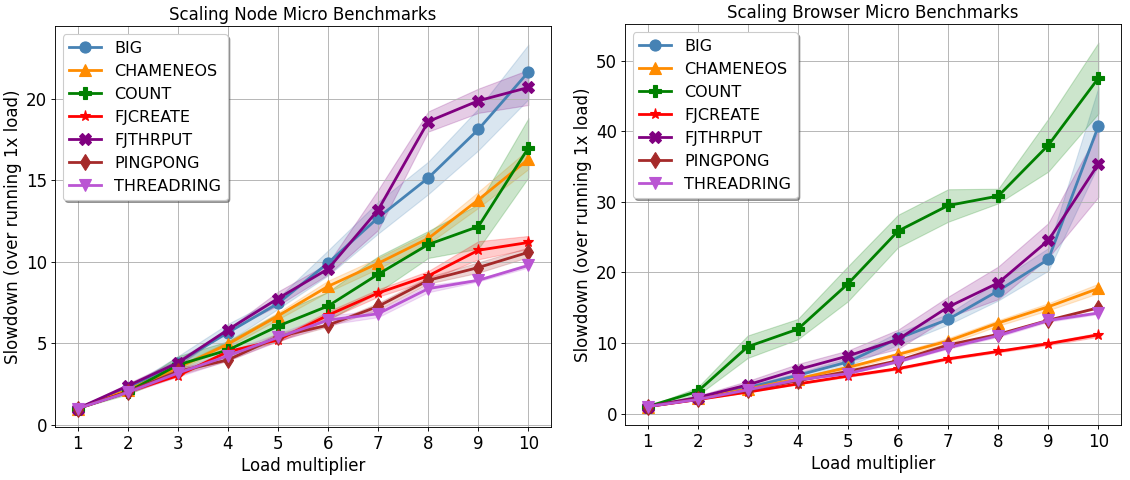
\includegraphics[width=\textwidth]{resources/load_scaling.png}
        \caption{Node.js and Browser Comparison for Micro-Benchmark Load Scaling}
    \end{centering}
\end{figure}
One can observe that big, chameneos, count and fork join throughput have the worst scaling when increasing load over both environments. All four of these involve large message queues, suggesting that JavaScript performs slower when more messages are in the event queue. The browser demonstrated approximately twice the slowdown for some of the benchmarks, which may be the result of less RAM being available on a browser instance than that of Node when queuing a large number of messages.
\subsection{Comparing Communication Links}
The Ping Pong and Fork Join (create) benchmarks were tested on a network using different links. In this comparison, the fork join benchmark only involves the remote spawning of actors without them executing any behaviour such as terminating. This way the comparison narrows down the performance to sending (ping pong) and remote spawning (fork join).
\begin{figure}[H]
    \begin{centering}
        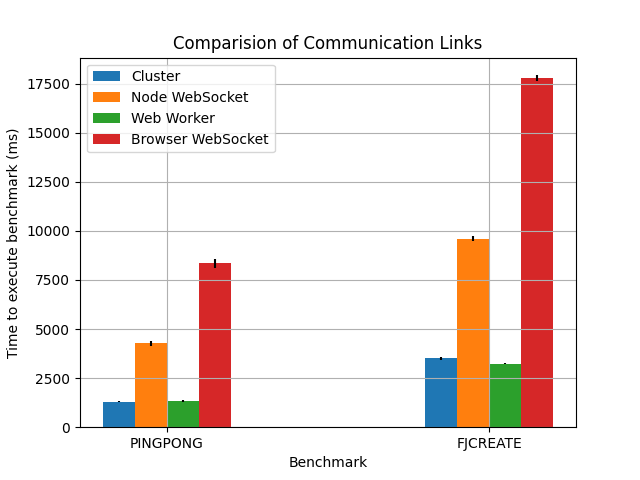
\includegraphics[width=270px]{resources/link.png}
        \caption{Comparison of Communication Links}
    \end{centering}
\end{figure}
Across both benchmarks, cluster and web workers are nearly identical in performance. Node.js uses an npm package to interface with the WebSocket server while the browser uses the available WebSocket functionality on JavaScript. The browser is slower when communicating through the WebSocket link in both cases. 

The WebSocket links are slower than the IPC alternative (Cluster and Web Workers) since they involve the network stack and introduce an additional network hop over the WebSocket server. Cluster and web workers use a direct link which is made between the spawner and the spawned worker; hence the message is not forwarded by an intermediary node. WebSocket performance would be improved if peer-to-peer connections between distributed instances were established.

Furthermore, the number of actors which are remotely spawned in fork join create is equal to the number of messages sent in the ping pong benchmark. The fork join benchmark is about twice as slow since it involves sending twice the number of messages over the network. The first message is a request sent to the remote instance to remotely spawn an actor. When the remote instance spawns the actor locally, it sends an acknowledgement message with the actor's address embedded within.
\subsection{Comparing with Existing Implementations}
\begin{figure}[H]
    \begin{centering}
        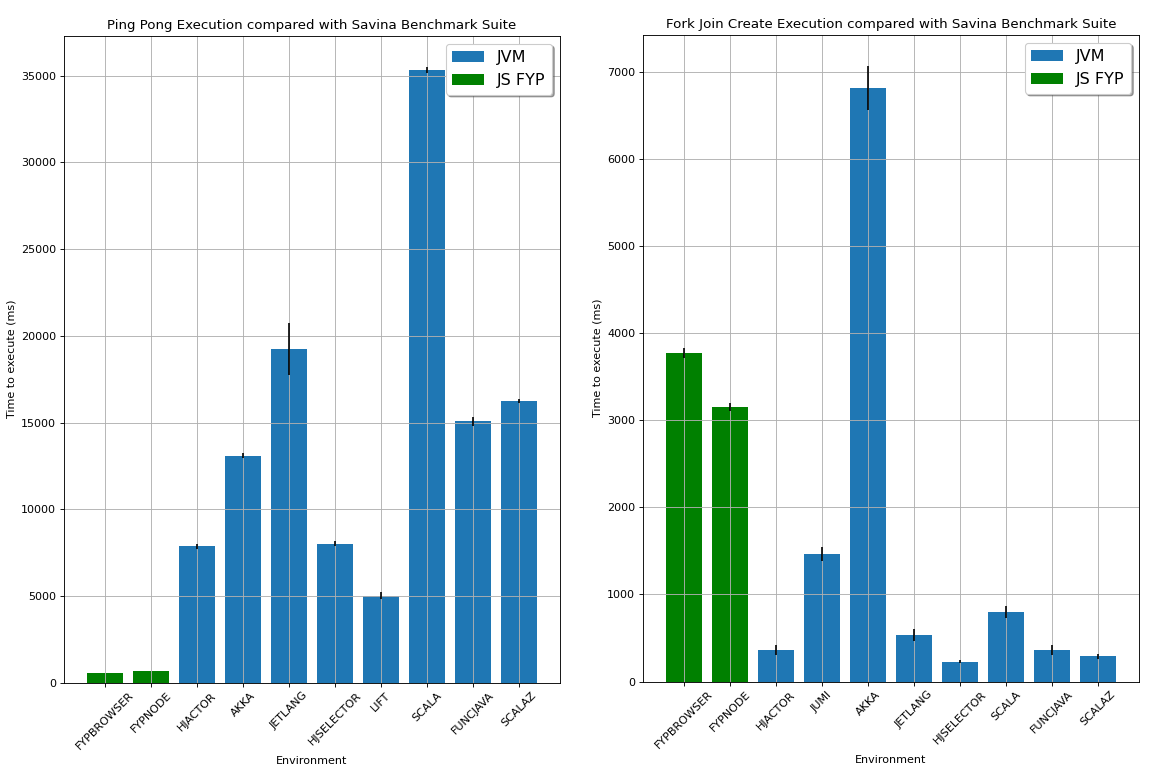
\includegraphics[width=\textwidth]{resources/savina.png}
        \caption{Savina Benchmark Comparison with Other Implementations}
    \end{centering}
\end{figure}
Our framework performs the fastest when messages are sent between actors. This is effectively the speed at which JavaScript can create and immediately resolve promises followed by minimal amount of work to create the next promise. Nact is much slower as it maintains a mailbox of messages using a queue and includes logic which checks if an actor is busy processing a message or not. This may be due to its features to persist actors and events on a database, which requires the framework to keep track of the current actor queues. Our framework benefits from acting as a wrapper around the event loop, as it directly makes use of the event queue to schedule tasks rather than performing the additional task of manipulating objects in memory. The JVM implementations prove to be more costly in general, where Scala required the throwing of exceptions~\cite{savina} to maintain the benchmark's control flow.

The framework does not perform as well when spawning actors, ranking in the fourth worst when compared with the JVM implementations and Nact.  Spawning actors in Nact ran much slower then our framework due to Nact's more complex logic involved when creating an actor which may be attributed to Nact's support for hierarchies of actors. Meanwhile our framework simply keeps record of the actor in a global object and returns the reference to that actor. Akka performed the slowest from JVM's category which is in line with the benchmarks executed in Savina's paper.  However, no reasons have been given for Akka's slow actor creation.

These benchmarks were also implemented for Spiders.js. This framework failed to create the number of actors spawned when benchmarking Fork Join Create (one million actors). This is due to the framework creating a new child process for each spawned actor to grant them their own thread of control, causing each actor to be memory intensive. Spiders.js was also dramatically slower when running the ping pong benchmark compared to its JavaScript and JVM counterparts. A modified version of a provided ping pong example was used to implement this benchmark, and poor processor utilisation was observed when sending messages between the actors involved. Running the benchmark also slowly and continuously allocated a considerable amount of RAM, which should not be the case when the number of actors is constant and not more than one message is queued at a time.
\section{Parallel Performance}
\subsection{Shared Memory Parallelism}
This subsection first demonstrates the parallel nature of the benchmarks and its results, followed by a mathematical explanation of each of the benchmarks.
\subsubsection{Performance Results}
The Savina benchmark suite includes parallel benchmarks where multiple actors perform computation in parallel to complete a task. Each of the explored parallel benchmarks benefit from master-worker parallelism, where a master actor farms tasks to worker actors which will start execution in parallel. The workers then report their results to the master which will aggregate the collected data, producing the final result. The framework is tested by first executing the benchmark using only one master and one worker in separate runtimes, where the worker is limited by JavaScript's single-threaded nature.  Next, two workers are spawned on separate runtimes, each of which ideally assigned half of the computational load by the master. Since the framework is tested on a system which houses four cores, the benchmarks are scaled up to four worker runtimes running in parallel. The amount of speedup introduced over running on one worker is tested and plotted below.
\begin{figure}[H]
    \begin{centering}
        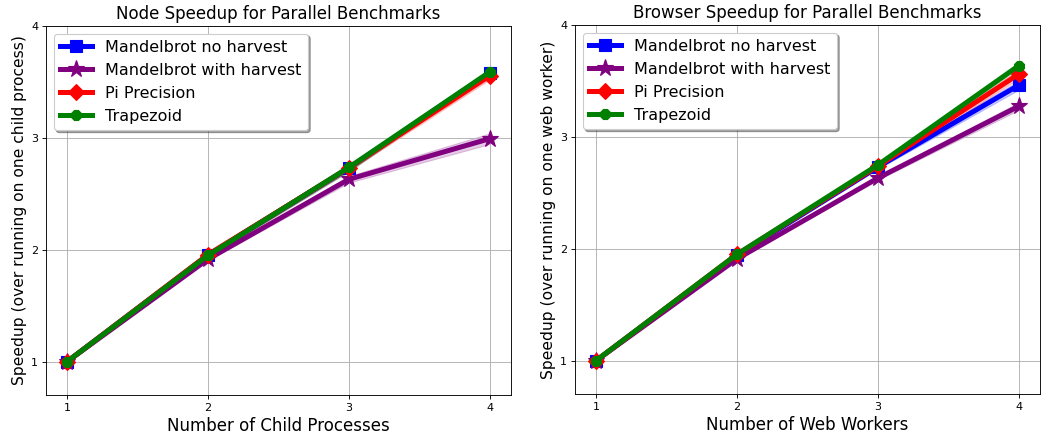
\includegraphics[width=390px]{resources/shared_memory_speedup.png}
        \caption{Node.js and Browser Comparison for Shared Memory Speedup}
    \end{centering}
\end{figure}
\subsubsection{Mandelbrot}
The Mandelbrot benchmark is not part of the Savina benchmark suite. Generating the Mandelbrot set is highly parallelisable as each pixel can be independently computed using a set of provided constants. 
\begin{itemize}
    \item The worker actors execute iterations of $z_{n+1}$ = $z_{n}^{2}+c$ where $z_0 = 0 + 0i$
    \item $c, z \in \mathbb{C}$. $n \in \mathbb{Z},$ $n \ge 0$
    \item $c$ is determined by the position of the pixel
    \item If $|z_n|> 2$ it is said to be unbounded and will generate a lighter pixel colour if $n$ is small. If it performs a set number of iterations and it is still bounded $(|z_n| \le 2)$, it will yield a darker colour.
\end{itemize}
Black pixels take longer to compute than white as the maximum number of iterations need to be performed to verify that it remains bounded. For this reason, Mandelbrot could not be split into even chunks amongst workers as chunks which have more black pixels would take considerably longer to execute, resulting in some workers finishing faster than others and thus reducing efficiency. The master could compose each task to be a single row where once a worker is finished with a row it is assigned the next required row. However, this would result in considerable message overhead as the number of messages exchanged between the master and its workers would be twice the image's height. A balance is struck between minimising message overhead and distributing even chunks by assigning smaller chunks to each worker. When the worker reports the results back it will be assigned the next required chunk.

When workers do not report back the generated pixels to the master, the speedup goes up to 3.5 with 4 running workers. The slowdown may be attributed to the fact that the master is running on its own process (thus using five processes on four cores) as well as any other processes and daemons running on the operating system which may have prevented the benchmark from fully utilising the CPU. The distributed chunk sizes may not have been optimal resulting in some workers finishing earlier than others, and there were instances where workers were idle while waiting for the next task to be assigned by the master. When harvesting the chunk's pixel data from the workers one can note that Node.js had more significant slowdown than the browser on four worker processes.
\subsubsection{Pi Precision and Trapezoidal Approximation}
The value of pi computation as well as the trapezoidal approximation benchmarks involve a master actor distributing iterations of mathematical computation to worker actors.

The value of pi is approximated using Equation~\ref{eq:1} which is defined by the Savina benchmark suite. The iterations of the summation can be distributed and parallelised amongst multiple worker actors.
\begin{equation} \label{eq:1}
\pi\approx\sum_{n=0}^{\infty}\left(\frac{4}{8n+1}-\frac{2}{8n+4}-\frac{1}{8n+5}-\frac{1}{8n+6}\right) \left(\frac{1}{16} \right)^n
\end{equation}
Trapezoidal approximation can also be distributed to perform the approximate integral of the following function specified by the Savina benchmark.
\begin{equation} \label{eq:2}
f(x)=\frac{1}{x+1}\cdot\sqrt{1+e^{\sqrt{2x}}}\cdot \sin\left(x^3-1\right)
\end{equation}
This is done by executing Equation~\ref{eq:3} with respect to $f(x)$. Each worker will execute smaller bounds of the integral of $f(x)$ which will be added up by the master to compute the full integral.
\begin{equation} \label{eq:3}
\int_{a}^{b}f(x)dx\approx\frac{b-a}{N}\left[ \frac{f(a)+f(b)}{2}+\sum_{k=1}^{N-1}f\left( a+k\cdot\frac{b-a}{N} \right) \right]
\end{equation}
\subsection{Distributed Memory Parallelism}
The following benchmark experiments with having actors hosted on a distributed memory. A Raspberry Pi 4 is used to host a WebSocket server which will handle the forwarding of messages between remote devices. The scaling of the Mandelbrot benchmark without harvesting pixel data over Node.js and browsers has already been explored up to four worker instances over shared memory. The diagram below shows the speedup introduced when connecting a new device on the network with the following specifications.
\begin{itemize}
    \item OS --- Windows 10 Home (64 bit)
    \item CPU --- Intel Core i5--10500 6 cores up to 3.10GHz with hyper-threading enabled
    \item RAM --- DDR4 32GB (4$\times$8GB) at 2666MHz
\end{itemize}
In addition to the four workers and master hosted on the four-core device, new workers are incrementally added and connected to the WebSocket server on the new device. While avoiding data harvesting to minimise the network dependency, one can observe a consistent speedup when adding more workers on the second device, with node achieving slightly better speedup with a larger number of workers. Despite network overhead being introduced when distributing actors over the network, the second device makes up for this with its faster processing time.
\begin{figure}[H]
    \begin{centering}
        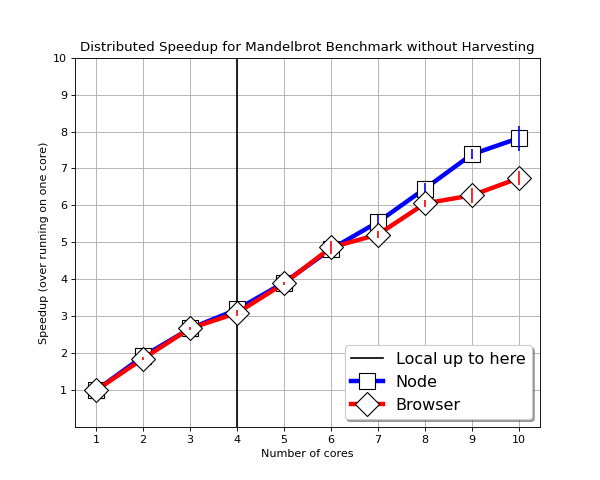
\includegraphics[width=300px]{resources/distributed_memory_speedup.png}
        \caption{Node.js and Browser Comparison for Distributed Memory Speedup}
    \end{centering}
\end{figure}
\section{Case Study}
While the qualitative analysis of the framework yielded sane results, the framework's ease of use is important for the developers making use of the API when engineering actor-based systems. This section focuses on two case studies which make use of the framework to create two communicating actors on a single instance as well as over a distributed network. The examples presented below work for both the Node.js and browser environments due to the framework implementations being fully interoperable.

The code segments below assume that the functions have been imported and that the actor behaviour is defined as follows.
\begin{lstlisting}    
import actors from 'actors.js';
const { init, spawn, spawnRemote, terminate, send} = actors

const pingPongBehaviour = (state, message, self) => {
    send(message.replyTo, {val: message.val-1, replyTo: self});
    if(message.val-1 < 0)
        terminate(self)
    else    
        console.log(message.val);
};
\end{lstlisting}
This code segment first imports the framework by using JavaScript ES6 imports. Lines 4--9 defines an actor behaviour which immediately sends a message to the sender including a reference to itself as well as the value it received subtracted by 1. It then checks if the value it received is less than 0, and if so the actor will terminate itself. Otherwise, it will output the received value. 
\subsection{Single Instance Actor Based System}
When making use of actors on a single instance, the developer is required to make use of three API functions taking in two parameters each. These functions allow the developer to \textbf{spawn} actors, \textbf{send} messages to them and \textbf{terminate} them to free up memory. The example below will make use of these three API functions to build two communicating actors for a specified load. Further information about using the API can be found in Appendix A.
\begin{lstlisting}    
const pingActorRef = spawn({}, pingPongBehaviour);
const pongActorRef = spawn({}, pingPongBehaviour);
send(pingActorRef, {replyTo: pongActorRef, val: 5});
\end{lstlisting}
Two actors are spawned with this behaviour, and the system is initialised by sending one of the actors the reference of the other actor as well as a value of 5. The first actor will output the values 5, 3 and 1 while the second actor will output the values 4 and 2, as they send each other decrementing values until both of which terminate when receiving a value of 0 or less.
\subsection{Distributing Parallel Actors over a Network}
The functionality demonstrated above can be replicated without the framework using function calls and JavaScript Promises. However, by using the actor framework API one can distribute the ping and pong actors across separate machines with minimal change in the code's logic. The provided WebSocket server needs to be started and set to expect three connected clients. 

One machine connects to the WebSocket server and uses the \textbf{spawnRemote} function instead of \textbf{spawn}, which requires an additional parameter to specify which remote machine will spawn the actor.
\begin{lstlisting}
init('ws://localhost:8080').then(async ready => {
    const pingActorRef = await spawnRemote(2, {}, pingPongBehaviour);
    const pongActorRef = await spawnRemote(3, {}, pingPongBehaviour);
    send(pingActorRef, {replyTo: pongActorRef, val: 5});
});
\end{lstlisting}

The two machines which will host ping and pong respectively will simply connect to the server.
\begin{lstlisting}
init('ws://localhost:8080')
\end{lstlisting}

Once all clients connect to the server, the server will lift the barrier and thus resolves the promise on the first machine. The first machine will send requests to spawn actors on the remote machines who only need to connect to the server. Due to location transparency, the \textbf{pingPongBehaviour} function remains unchanged, as the framework internally resolves which communication link needs to be used when replying to the actor. In this case, the actors will communicate with each other over the WebSocket link.

The developer can pass in additional parameters to specify the timeout to wait for the server to lift the barrier, as well as how many additional Web Workers or Node.js Child Processes it should spawn and connect to the WebSocket network. The code segment below spawns the ping actor on one spawned worker and the pong actor on another. This is done by passing additional parameters to the \textbf{init} function. The spawned workers take the form of Web Workers or Child Processes depending on the environment it is run on.
\begin{lstlisting}
init('ws://localhost:8080', 10000, 2).then(async ready => {
    if(ready.yourNetworkNumber === 1){
        const pingActorRef = await spawnRemote(2, {}, pingPongBehaviour);
        const pongActorRef = await spawnRemote(3, {}, pingPongBehaviour);
        send(pingActorRef, {replyTo: pongActorRef, val: 5});
    }
});
\end{lstlisting}
With this simple change, the actors now communicate through each other using IPC through the primary node to avoid the WebSocket server additional hop and network stack. An if statement is placed as each spawned worker will run the same code segment, and only one node should be remote spawning to other nodes.

This section demonstrates the minimal code changes required to scale an application from a single instance to using a distributed network or a multicore system through the use of only five API functions.
\chapter{Conclusions and Future Work}
The prototype successfully provides an intuitive, scalable, and fairly performant JavaScript implementation of the actor model for both the Node.js and browser environments. The functionality is exposed through an API as a collection of functions which abstract the concept of actors as well as the use of numerous communication links for distributed and parallel programming. The developed framework exploits the similarities between Gul Agha's~\cite{agha1985actors} definition of the actor model and JavaScript's event loop~\cite{eventloopbrowser}\cite{eventloopnode} to minimise the slowdown introduced when utilising the framework. 

Each of the dissertation's four objectives have been fully completed. The two frameworks allow developers to spawn and send messages to actors on local Node.js and browser instances respectively. Messages are processed through the execution of the predefined behaviour of actors (objective 1). Using several web technologies, developers are not limited to a single instance when spawning actors, as they can remotely spawn actors on remote browsers and Node.js instances (objective 2). Once actors are spawned either locally or remotely, the framework internally handles local and remote communication without additional input required by the user (objective 3, location transparency).

Qualitative benchmarks yielded sane results when using the Savina actor benchmark suite~\cite{savina}. The separate Node.js and browser frameworks demonstrated similar performance in most cases with reasonable standard error, and the provided communication links perform consistently across the different benchmarks. The performance of the prototype is compared with existing JavaScript and JVM implementations, achieving the fastest times for sending messages between actors and having them subsequently processed. The speedup of parallel actors was observed to be close to the ideal linear speedup when utilising up to four cores and achieves a reasonable speedup when distributed actors are introduced. 

The developed actor framework is not without its limitations. Distributed clients must connect to a provided WebSocket server to communicate with their peers. Each client must wait for the expected number of clients to connect before being allowed to communicate with each other, and communication over the server introduces an intermediary network hop. The distribution of actors could be done using peer-to-peer WebSocket connections at the cost of more complex synchronisation and requiring each client to listen for connections.

The framework also lacks quality of life features such as the ability to freeze actors and persist them to a file. Persisted actors could then be spun up in different environments or runtimes or serve as backup for when an actor reaches an undefined state. The framework could also provide means to implement a hierarchy of actors, where the termination of an actor would automatically terminate its children, or have actors supervise other actors to provide fault tolerance.

Grounded in the actor model's theory, the prototype compliments the internet's distributed environment made up of machines hosting multicore processors, while taking advantage of JavaScript's far-reaching availability through the use of server-side applications and browsers. It provides a solution for developers to fully utilise the hardware present in multiple devices running vastly different operating systems with varying restrictions, given that a compatible browser is present.
\appendix
\chapter{Manual}
This section explores each of the functions that the framework exposes which developers will interact with to make use of the actor model in JavaScript. Using ES6 Modules the functions are imported as follows.
\begin{lstlisting}
import actors from 'actors.js';
const { init, spawn, spawnRemote, terminate, send} = actors
\end{lstlisting}
\section{Spawning Local Actors}
When the developer calls the \textbf{spawn} function, they will pass in the actor's initial state as the first parameter. The actor will maintain this state throughout every processed message and it can be manipulated by its behaviour. As a second parameter the developer must specify the actor's behaviour which has the actor's current state, current processed message as well as the actor's self reference as parameters. Using these parameters, the developer can define how the behaviour should manipulate the actor's state or how the message contents should be processed. It also allows the actor to pass a reference of itself to other actors using the behaviour's third parameter.

The example below defines the actor behaviour to print out each of the parameters. This function is used to spawn an actor with that behaviour, and a reference to that actor is returned.
\newpage
\begin{lstlisting}
// Actor behaviour
const pongBehaviour = (state, message, self) => {
    console.log("My state object is " + state);
    console.log("I'm processing the message object " + message);
    console.log("Actor self reference " + self);
};

//Spawn an actor with the above behaviour and an initial state
const pongReference = spawn({stateElement: "hello"}, pongBehaviour);
\end{lstlisting}
Note that with this implementation nothing is printed out, as the actor behaviour is only executed in response to a message which is sent to the spawned actor.
\section{Sending Messages to Actors}
The \textbf{send} function is used to send a message to an actor. It takes in the actor reference and message object to send as parameters.
\begin{lstlisting}
send(pongReference, {messageVal: "This is a message!"});
\end{lstlisting}
One of the framework's key features is location transparency. The framework internally identifies the fastest medium to use for message transportation and sends the message through that link.
\section{Terminating Actors}
An actor can be terminated using the \textbf{terminate} function. The function takes in the actor to terminate as the first parameter. The actor will process its remaining queued messages as these are events already queued in the browser or Node.js's event loop. To forcefully terminate an actor, the second parameter can be set to true which will deactivate the actor. When the remaining messages are processed, the actor will perform minimal work ignoring the messages.
\begin{lstlisting}
terminate(pingReferece, false)      //forceful termination
terminate(pongReference, false)     //non-forceful termination
\end{lstlisting}
\section{Connecting Processes to the Network}
The \textbf{init} function handles the spawning of worker processes as well as connections with other Node.js and browser runtimes through WebSockets.
\begin{lstlisting}
//Connect to local WebSocket server and spawn four processes. Wait 10000ms for all processes to connect
init('ws://localhost:8080', 10000, 4).then(ready => {
    if (ready.yourNetworkNumber === 1) {
        //Code for node 1 to execute
    }
})
\end{lstlisting}
 
The first parameter takes in the URL of the WebSocket server. The second parameter is the timeout, which defines how long the client will wait for all clients to connect to the network. The third and final parameter is the number of workers that are to be spawned. Each of these workers will connect to the WebSocket server.

Once all clients connect to the server, the server broadcasts a message indicating that it is ready to receive and forward communication between connected clients. This message has embedded within it information about the connected clients' IP addresses and unique incrementally assigned network numbers, as well as the network number assigned to the client receiving the message. In the example above, four processes are spawned (given network numbers 2 to 5), so an if statement is used to define logic only executed by the primary process possessing network number 1.

\section{Remotely Spawning Actors}
After invoking \textbf{init}, the developer can use \textbf{spawnRemote} to remotely spawn actors in other connected clients. This function takes the network number of the client to spawn the actor on as the first parameter, the initial state as the second parameter and the actor behaviour as the final parameter.
\newpage
\begin{lstlisting}
const pingPongBehaviour = (state, message, self) => {
    console.log(message.val);
    if(!(message.val-1 < 0))
        send(message.replyTo, {val: message.val-1, replyTo: self});
};
//Specify timeout and number of workers to spawn
init('ws://localhost:8080', 10000, 2).then(async ready => {
    //The primary node always connects first
    if(ready.yourNetworkNumber === 1){
        const ping = await spawnRemote(2, {}, pingPongBehaviour);
        const pong = await spawnRemote(3, {}, pingPongBehaviour);
        //Send ping a message. Output will be decrementing values from 5 to 0
        send(ping, {replyTo: pong, val: 5})
    }
});
\end{lstlisting}
In the example above, nodes 2 and 3 are the workers that the primary node spawned. Node 1 sends requests to its peers to spawn actors with a specific behaviour and initial state. The \textbf{spawnRemote} function returns a Promise which is resolved once the actor is remotely spawned and an acknowledgement is returned. The promise resolves into an actor reference which has embedded information indicating that this is a remote node. This enables location transparency when sending to the actor, as the developer need not be aware of whether the actor reference points to a local or remote actor, as communication is handled internally by the framework.


\bibliomatter
\raggedright
\bibliographystyle{ieeetr}
\bibliography{references}
 
\end{document}